\section{Resoconto delle attività di verifica} \label{res verifica}
	Questa sezione illustra i risultati di verifica ottenuti utilizzando 
	le metriche esposte nella sezione §\ref{subsec:metriche} nel corso
	dello sviluppo del progetto (per la spiegazione dei diversi periodi vedere 
	in \vPianoDiProgetto{}).
	Le misurazioni sono state fatte a distanza di sette giorni l'una dall'altra e
	vengono presentate con un diagramma, che fa da cruscotto,
	per evidenziare le variazioni nel tempo. È stato scelto il diagramma a cruscotto perché 
	più parlante rispetto alla classica rappresentazione tabellare per gli esiti delle verifiche.\\
	
	\subsection{Verifica dei processi}
		\subsubsection{Cost Variance}
	
		\begin{figure}[H]{\textwidth}
  			\centering
  			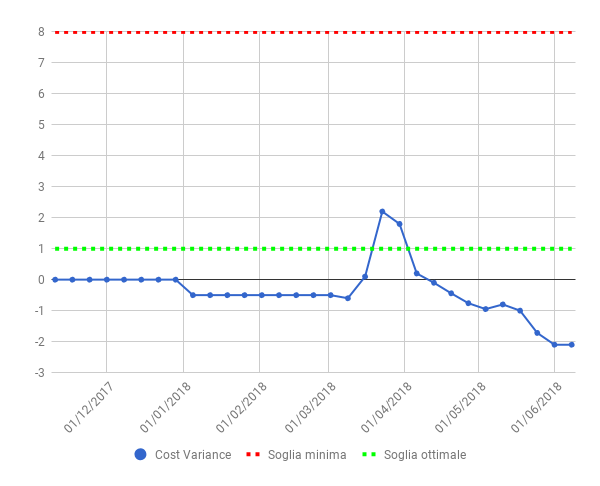
\includegraphics[width=1\linewidth]{./img/Risultati/CostVariance.png}
	  		\caption{Variazione della metrica Cost Variance}
		\end{figure}\\
		
		Questa metrica è strettamente dipendente con la Schedule Variance infatti,  
		se un'attività termina prima del tempo previsto, la Cost Variance diminuisce
		perché il monte ore preventivato per quell'attività è superiore alle ore 
		effettive. Quindi, nel grafico precedente, una diminuzione della Cost Variance
		corrisponde ad attività terminata in anticipo mentre un aumento corrisponde
		ad un ritardo nei tempi previsti.\\
				
		\subsubsection{SPICE}
		\begin{figure}[H]{\textwidth}
			\centering
			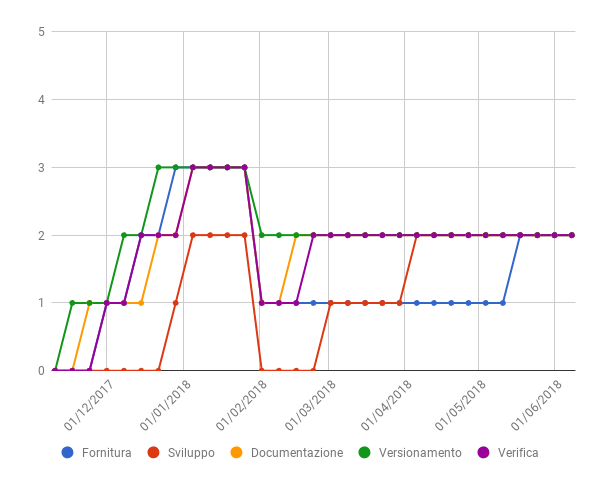
\includegraphics[width=1\linewidth]{./img/Risultati/SPICE.png}
			{\footnotesize Il calo a seguito alla \RR{}(2018-01-26) 
			è causato da una rivalutazione del livello raggiunto e non
			da una effettiva perdita di maturità dei processi.
			\par}
			\caption{Variazione dei valori SPICE}
		\end{figure}

\newpage
		
		\subsubsection{Schedule Variance}
			Questi risultati hanno una rappresentazione tabellare perché, per come
			é definita la Schedule Variance (descritta nelle \vNormeDiProgetto{}), i valori 
			sono relativi alle diverse attività presenti nei diversi periodi, descritti nel
			\vPianoDiProgetto{}, e vengono quindi calcolati solamente a fine del periodo e non 
			durante questo.		
		
		\begin{center}
   			\begin{longtable}{ | >{\raggedright\arraybackslash}m{5cm} | >{\centering\arraybackslash}m{5cm} | }
        
        	\hline
        		\textbf{Attività} & \textbf{Schedule Variance} \\ \hline
        	\endhead
        		Analisi dei Requisiti	 & $0$\\ \hline
        		Glossario	& $0$ \\ \hline
        		Norme di progetto	& $0$\\ \hline
        		Piano di progetto	& $0$\\ \hline
        		Piano di qualifica	& $-2$\\ \hline
        		Studio di fattibilità& $0$\\ \hline 
        		\hline
        		\textbf{Totale} & $-2$\\\hline
			\caption[Schedule Variance - Analisi, analisi in dettaglio]{Schedule Variance nel periodo di analisi e analisi in dettaglio}
			\end{longtable}
	
		\end{center}
	  		
	  	\begin{center}
   			\begin{longtable}{ | >{\raggedright\arraybackslash}m{5cm} | >{\centering\arraybackslash}m{5cm} | }
        
        	\hline
        		\textbf{Attività} & \textbf{Schedule Variance} \\ \hline
        	\endhead
        		Incremento documenti precedenti	 & $+1$\\ \hline
        		Tecnology baseline	& $-2$ \\ \hline
        		\hline
        		\textbf{Totale} & $-1$\\\hline
			\caption[Schedule Variance - Progettazione architetturale]{Schedule Variance nel periodo di Progettazione architetturale}
			\end{longtable}
	
		\end{center}
		
		\begin{center}
   			\begin{longtable}{ | >{\raggedright\arraybackslash}m{5cm} | >{\centering\arraybackslash}m{5cm} | }
        
        	\hline
        		\textbf{Attività} & \textbf{Schedule Variance} \\ \hline
        	\endhead
        		Incremento documenti precedenti	 & $+1$\\ \hline
        		\glossaryItem{Product baseline}	& $+1$ \\ \hline
        		Manuale utente	 & $0$\\ \hline
        		Manuale sviluppatore	& $+1$ \\ \hline
        		Codifica	 & $-5$\\ \hline
        		\hline
        		\textbf{Totale} & $-2$\\\hline
			\caption[Schedule Variance - Progettazione in dettaglio e codifica]
				{Schedule Variance nel periodo di Progettazione in dettaglio e codifica}
			\end{longtable}
	
		\end{center}
		
		\begin{center}
   			\begin{longtable}{ | >{\raggedright\arraybackslash}m{5cm} | >{\centering\arraybackslash}m{5cm} | }
        
        	\hline
        		\textbf{Attività} & \textbf{Schedule Variance} \\ \hline
        	\endhead
        		Incremento documenti precedenti	 & $+1$\\ \hline
        		Esecuzione dei test	& $-2$ \\ \hline
        		Correzione bug	 & $-3$\\ \hline
        		Collaudo	& $-1$ \\ \hline
        		\hline
        		\textbf{Totale} & $-5$\\\hline
			\caption[Schedule Variance - Validazione e collaudo]
				{Schedule Variance nel periodo di Validazione e collaudo}
			\end{longtable}
	
		\end{center}
	
	\subsection{Verifica dei prodotti}
		\subsubsection{Indici Gulpease}
		
		\begin{figure}[H]{\textwidth}
  			\centering
  			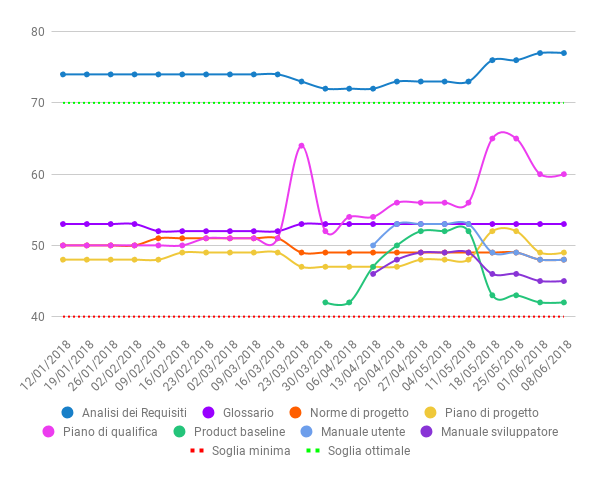
\includegraphics[width=1\linewidth]{./img/Risultati/Gulpease.png}
	  		\caption[Variazione indici Gulpease]{Variazione degli indici Gulpease nei documenti}
		\end{figure}
		
		\subsubsection{Grado di accoppiamento}
	
		\begin{figure}[H]{\textwidth}
  			\centering
  			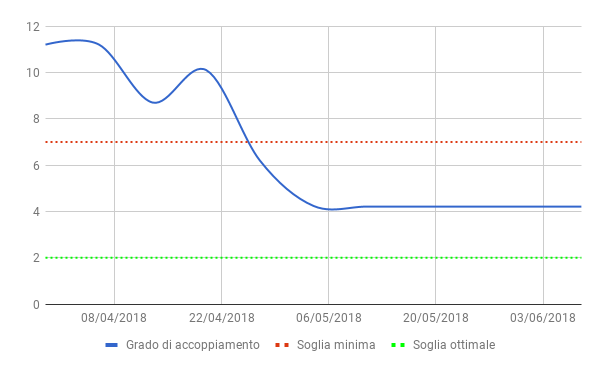
\includegraphics[width=1\linewidth]{./img/Risultati/Coupling.png}
	  		\caption{Variazione della metrica Grado di accoppiamento}
		\end{figure}\\
		
		\subsubsection{Code Coverage}
		
		\begin{figure}[H]{\textwidth}
  			\centering
  			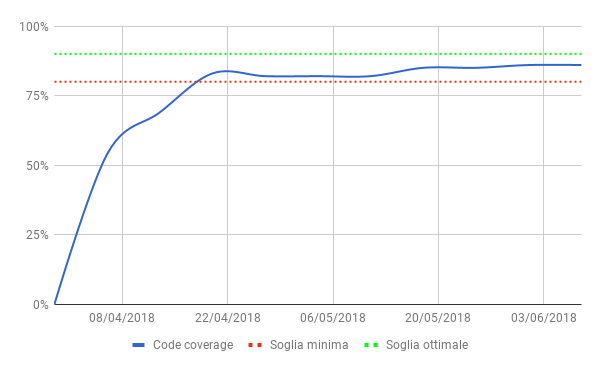
\includegraphics[width=1\linewidth]{./img/Risultati/CodeCoverage.png}
	  		\caption[Variazione Code Coverage]{Variazione della metrica Code Coverage}
		\end{figure}
		
		\subsubsection{Rapporto linee di commento per linee di codice}
		
		\begin{figure}[H]{\textwidth}
  			\centering
  			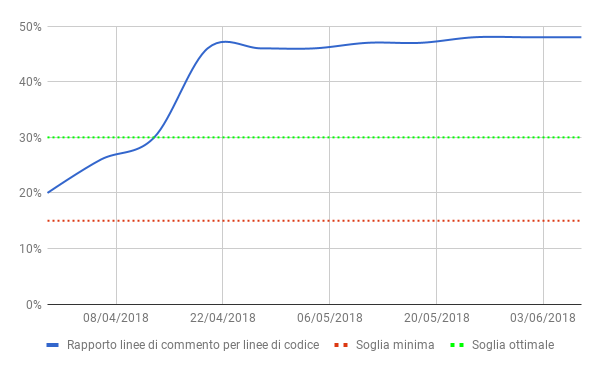
\includegraphics[width=1\linewidth]{./img/Risultati/RapportoCommentoCodice.png}
	  		\caption[Variazione rapporto linee di commento per linee di codice]{Variazione del rapporto tra le linee di commento e quelle di codice}
		\end{figure}
		
		\subsubsection{Complessità ciclomatica}
		
		\begin{figure}[H]{\textwidth}
  			\centering
  			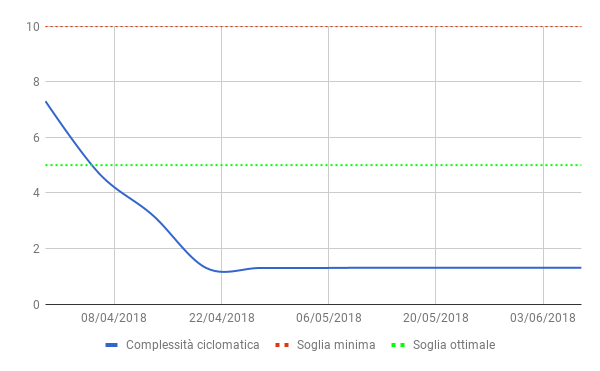
\includegraphics[width=1\linewidth]{./img/Risultati/ComplessitaCiclomatica.png}
	  		\caption[Variazione complessità ciclomatica]{Variazione della complessità ciclomatica del prodotto}
		\end{figure}
		
		\subsubsection{Percentuale superamento test}
		
		\begin{figure}[H]{\textwidth}
  			\centering
  			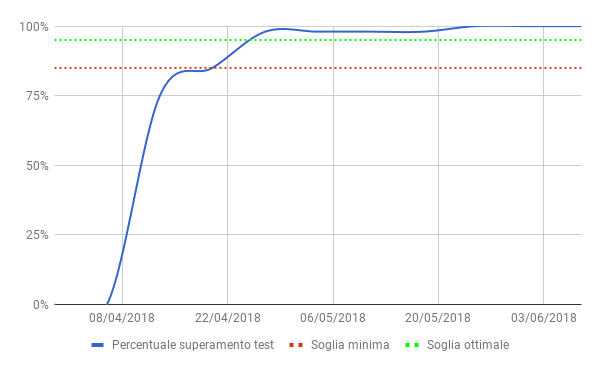
\includegraphics[width=1\linewidth]{./img/Risultati/SuperamentoTest.png}
	  		\caption[Variazione percentuale superamento dei test]{Variazione della percentuale di superamento dei test}
		\end{figure}
		
		\subsubsection{Requisiti obbligatori soddisfatti}
		
		\begin{figure}[H]{\textwidth}
  			\centering
  			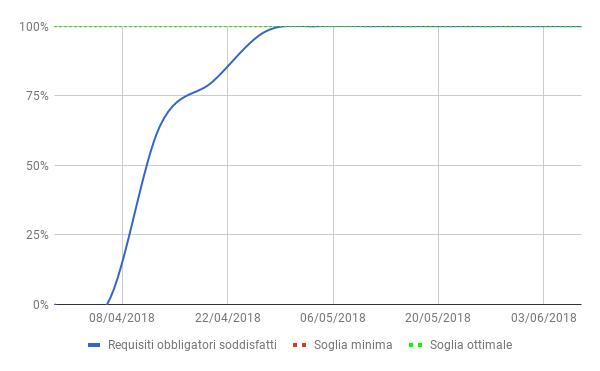
\includegraphics[width=1\linewidth]{./img/Risultati/RequisitiObbligatoriSoddisfatti.png}
	  		\caption[Variazione requisiti obbligatori soddisfatti]{Variazione della percentuale di requisiti obbligatori soddisfatti}
		\end{figure}
